\documentclass[aspectratio=169]{beamer}
\usepackage[utf8]{inputenc}
\usepackage[T2A]{fontenc}
\usepackage[ukrainian]{babel}
\usepackage{../templates/ITMOtheme}
\usepackage{tikz}

\title{Рубіжний контроль}

\author{Хмарук О. Ю.}

\where{Київ}
\date{2025}

\subject{Інформаційні системи}

\begin{document}

\begin{frame}[plain]
  \titlepage
\end{frame}

\section{Вступ}

\begin{frame}
\frametitle{Тема роботи}
  Використання систем управління вмістом (CMS)\footnote{CMS -- програмне забезпечення для створення, редагування, організації та публікації цифрового контенту. Забезпечує централізоване управління даними через веб-інтерфейс без необхідності програмування.} для розробки ігор
\end{frame}

\begin{frame}
\frametitle{Актуальність проблеми (1)}

  \begin{itemize}
    \item Ігрові проєкти оперують специфічними форматами даних: скелетні анімації (Spine), спрайтшити, растрові шрифти, 3D-моделі
    \item Традиційні CMS (WordPress, Directus, Strapi, Sanity) орієнтовані на веб-контент
    \item Контент-менеджери та геймдизайнери змушені працювати через файлові системи, таблиці або кастомні внутрішні інструменти, що призводить до втрати продуктивності та помилок
    \item Відсутність єдиної системи для управління ігровими ресурсами створює бар'єр між технічними та нетехнічними учасниками команди
  \end{itemize}
\end{frame}

\begin{frame}
\frametitle{Актуальність проблеми (2)}

  \begin{itemize}
    
    \item Формати, специфічні для ігор (спайтшит, скелетні анімації, растрові шрифти), будуються на взаємопов'язаних файлах. Наприклад, спайн анімація:
    \bigskip
  
    \begin{center}
      \begin{tikzpicture}[node distance=1.5cm, every node/.style={rectangle, draw, rounded corners, font=\small, fill=white, align=center}]
        \node (skeleton) {Скелетон \\ (animation.json)};
        \node (atlas) [right=2.5cm] {Атлас \\ (animation.atlas)};
        \node at (2, -2) (textures1) {Текстури \\ (animation1.png)};
        \node at (5, -2) (textures2) {Текстури \\ (animation2.png)};
        \draw[->, thick] (skeleton) -- (atlas);
        \draw[->, thick] (atlas) -- (textures1);
        \draw[->, thick] (atlas) -- (textures2);
      \end{tikzpicture}
    \end{center}

    \bigskip

    Опис таких взаємозв'язків є нетривіальною задачею для традиційних CMS.
  \end{itemize}
\end{frame}

\begin{frame}
  \frametitle{Постановка задачі}

  \begin{itemize}
    \item Спроєктувати компонентну систему для опису довільних сутностей
    \item Реалізувати систему зберігання файлів із підтримкою локального сховища та S3-сумісних провайдерів \footnote{S3 -- сервіс об'єктного зберігання від Amazon Web Services, який дозволяє масштабовано зберігати та отримувати будь-які дані через HTTP API.}
    \item Створити плагінну архітектуру, що дозволяє розширювати систему компонентами
    \item Розробити веб-дашборд для візуального управління сутностями та файлами
    \item Забезпечити типобезпечний API для інтеграції з ігровими рушіями
  \end{itemize}
\end{frame}

\begin{frame}
\frametitle{Існуючі аналоги}
  \begin{table}
    \footnotesize
    \begin{tabular}{l|c|c|c|c}
      \textbf{Критерій}                   & \textbf{Strapi} & \textbf{Sanity} & \textbf{Contentful} & \textbf{Game CMS} \\
      \hline
      Ігрові формати (Spine, Spritesheet) & ---             & ---             & ---                 & + \\
      Прев'ю ігрових ресурсів             & ---             & ---             & ---                 & + \\
      Чернетки / Публікації               & +               & +               & +                   & + \\
      Плагінна архітектура                & частково        & +               & частково            & + \\
      Self-hosted                         & +               & ---             & ---                 & + \\
      MongoDB                             & ---             & власна БД       & хмара               & + \\
      Типобезпечний API                   & частково        & частково        & частково            & + \\
      Компонентна вкладеність             & обмежена        & +               & обмежена            & + \\
    \end{tabular}
  \end{table}
\end{frame}

\begin{frame}
\frametitle{Методи рішення}
  \begin{itemize}
    \item Для зберіння даних використаємо мокументо-орієнтовану БД (MongoDB) -- гнучка схема для довільних структур сутностей без міграцій, при зміні схеми.
    \item Кожен тип даних описується як незалежний компонент із валідацією, серіалізацією та пошуковим індексуванням
    \item Для розширення створимо плагінну систему, яка зможе додавати нові компоненти, маршрути API, сторінки дашборду, типи файлів
    \item Для сховища файлів створимо абстракція Storage Provider для заміни реалізації (Local / S3) без зміни бізнес-логіки
  \end{itemize}
\end{frame}

\begin{frame}
\frametitle{Архітектура системи}

  \begin{figure}
    \centering
    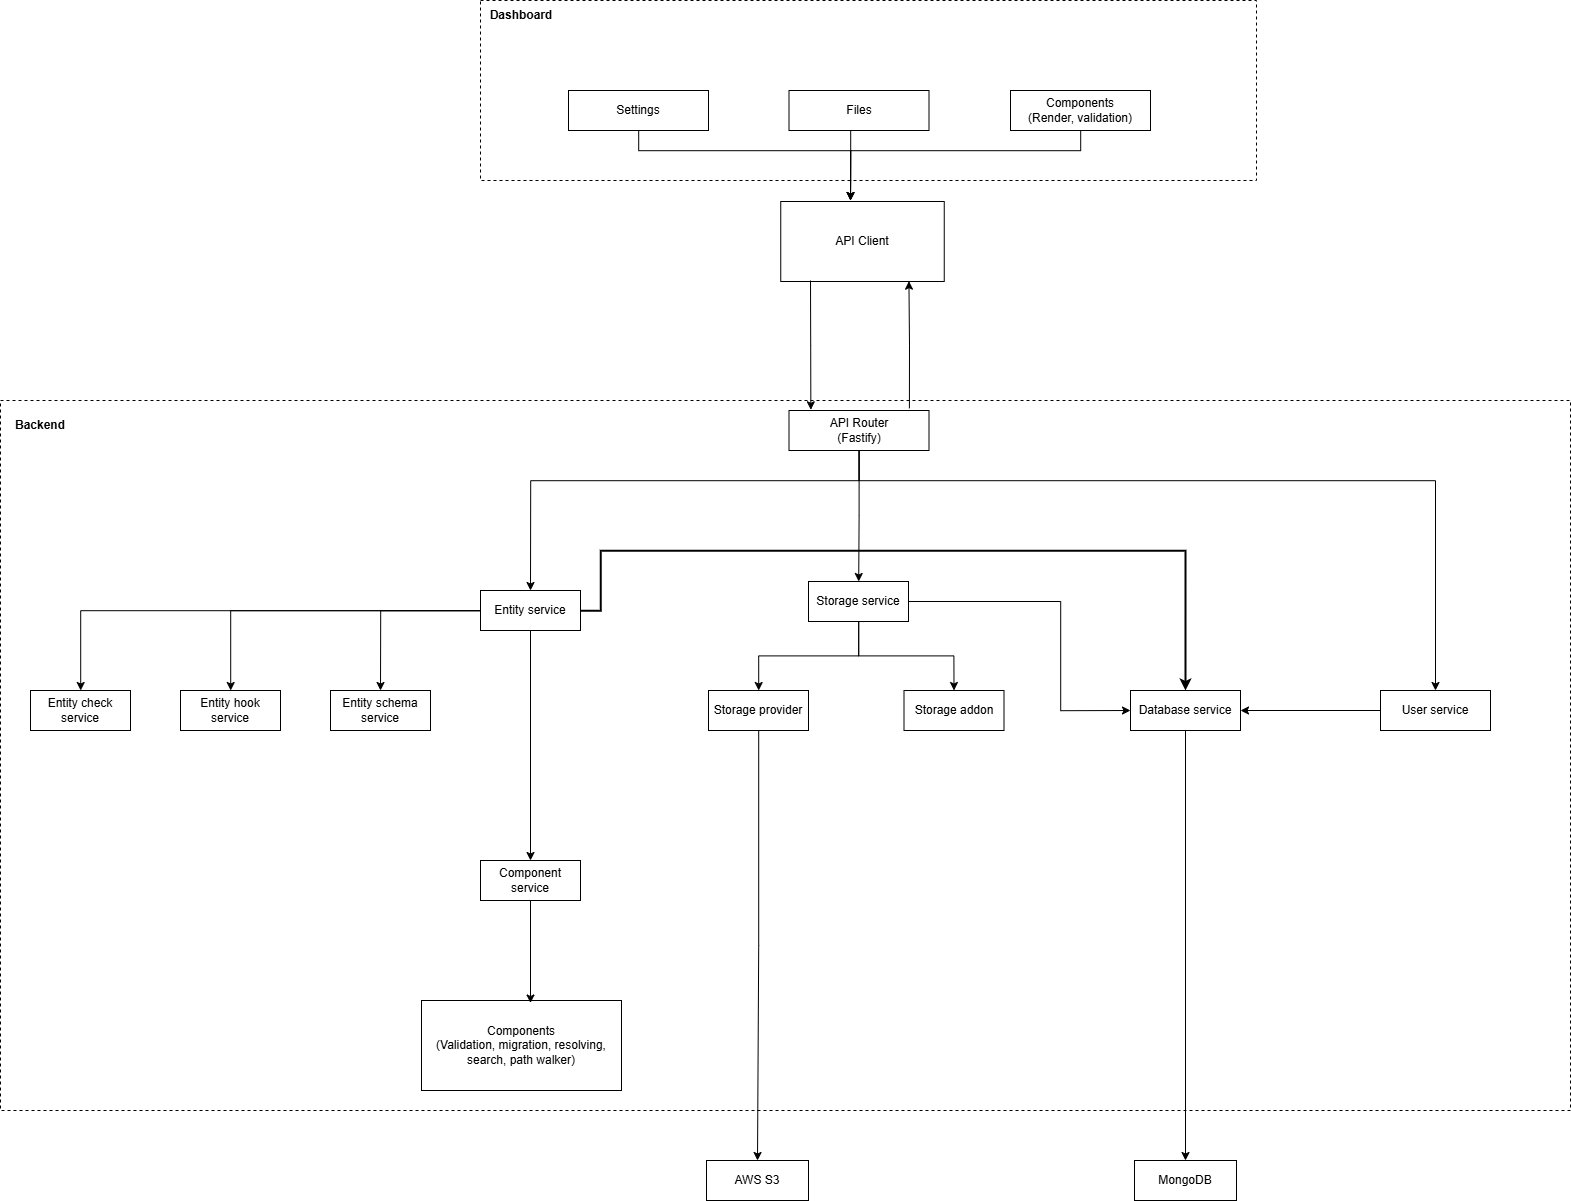
\includegraphics[height=2.5in]{media/arch.png}
    \caption{Архітектура системи CMS}
  \end{figure}
\end{frame}

\begin{frame}
\frametitle{Компонентна система (1)}

  Кожен компонент має різні види даних на різних етапах:

  \begin{itemize}
    \item out -- дані, які повертаються з REST API
    \item in -- дані, які приймає REST API
    \item client -- дані, які зберігаються на клієнті
    \item storage -- дані, які зберігаються в БД
    \item resolved - дані, які повертаються при передачі допоможних аргументів
    \item searchIndex -- допоміжні дані для пошуку, які зберігаються в БД
  \end{itemize}
\end{frame}

\begin{frame}
\frametitle{Компонентна система (2)}

  Кожен компонент описується чітко визначеним інтерфейсом:

  \begin{itemize}
    \item \textbf{core} -- ідентифікатор, валідатор, значення за замовчуванням
    \item \textbf{controller} -- міграція та структура даних
    \item \textbf{storageTransformer} -- серіалізація даних для зберігання в MongoDB
    \item \textbf{clientTransformer} -- перетворення даних для клієнта
  \end{itemize}
\end{frame}

\begin{frame}
\frametitle{Компонентна система (3)}

  \begin{figure}
    \centering
    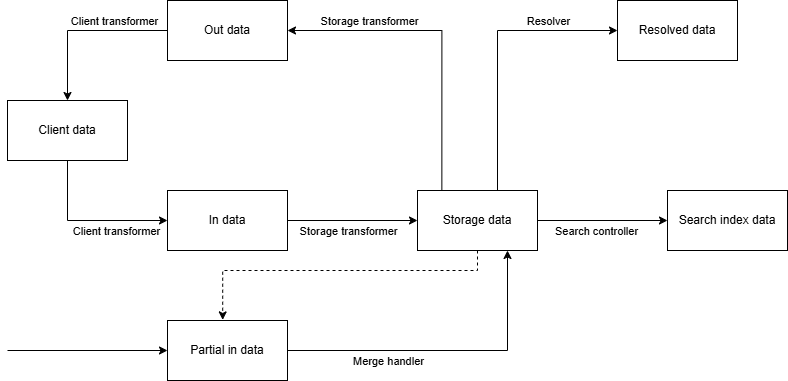
\includegraphics[height=2.25in]{media/data-flow.png}
    \caption{Діграма перетворення даних}
  \end{figure}
\end{frame}

\begin{frame}

\frametitle{Компонентна система (4)}

  Розділимо компоненти на такі типи:

  \begin{itemize}
    \item Контейнери -- містять в собі будь-які компоненти
    \item Примітиви - містять в собі нероздільний тип даних
    \item Складні -- містять передвизначену кількість інших компонентів
  \end{itemize}

  \begin{table}
    \footnotesize
    \begin{tabular}{l|l|l}
      \textbf{Контейнери} & \textbf{Примітиви} & \textbf{Складні} \\
      \hline
      Compose     & Text           & File \\
      Alternative & Number         & Font \\
      Repeatable  & Checkbox       & EntityReference \\
      DynamicZone & Date           &  \\
      Graph       & Dropdown       &  \\
                  & Json           &
    \end{tabular}
  \end{table}
\end{frame}

\begin{frame}
\frametitle{Компонентна система (5)}

  Для опису ігрових сутностей додамо наступні компоненти:

  \begin{description}
    \item[Spine] — скелетна анімація: атлас, скелет, текстури; генерація тіньового атласу для прев'ю; множинні текстури для варіантів персонажів
    \item[Spritesheet] — спрайтшити: текстура + JSON-атлас; обробка через Sharp; валідація через PixiJS
    \item[BitmapFont] — растрові шрифти: SDF-формат для масштабування; метадані + текстура
    \item[ThreeDModel] — 3D-моделі: GLB (GLTF Binary) формат;
  \end{description}
\end{frame}

\begin{frame}
\frametitle{Система зберігання файлів}

  \begin{itemize}
    \item Ієрархічна організація -- файли та папки з батьківськими посиланнями
    \item Presigned URLs -- пряме завантаження на S3 з клієнта без проксювання через сервер
    \item Addon-система -- обробка файлів після завантаження (мініатюри, метадані зображень)
    \item File Tracing -- відстеження, які сутності посилаються на які файли
    \item Плагінні прев'ю -- рендеринг попереднього перегляду для кастомних типів файлів
  \end{itemize}
\end{frame}

% \begin{frame}
% \frametitle{Механізм чернеток та публікацій}
%   \begin{center}
%     Створення $\rightarrow$ \textbf{[Draft]} $\rightarrow$ Публікація $\rightarrow$ \textbf{[Published]} $\rightarrow$ Скасування $\rightarrow$ \textbf{[Draft]}
%   \end{center}% 

%   \bigskip
%   \begin{itemize}
%     \item Кожна сутність має \textbf{draft} та опціональний \textbf{published}
%     \item Редагування виключно в draft — опублікована версія залишається стабільною
%     \item \textbf{Entity Checks} — кастомна валідація перед публікацією
%     \item \textbf{Entity Hooks} — вебхуки на події для інтеграції з ігровими серверами та CI/CD
%     \item Пошукова система індексує дані на рівні компонентів із порогом релевантності 0.8
%   \end{itemize}
% \end{frame}

\section{Результати}

\begin{frame}
\frametitle{Поточний стан розробки}

  \begin{itemize}
    \item Ядро CMS із компонентною системою (15 базових + 4 ігрових компоненти)
    \item REST API на Fastify
    \item Веб-дашборд
    \item Система файлів з підтримкою локального та віддаленого зберігання (S3)
    \item Механізм чернеток/публікацій із хуками та перевірками
    \item Плагінна архітектура з ігровим плагіном
  \end{itemize}
\end{frame}

\begin{frame}
\frametitle{Висновки}

  \begin{itemize}
    \item Розроблено спеціалізовану CMS для управління ігровим контентом
    \item Компонентна архітектура забезпечує гнучкість опису довільних сутностей
    \item Плагінна система дозволяє розширювати функціональність без модифікації ядра
    \item Типобезпечний API гарантує коректність даних на всіх рівнях
  \end{itemize}

\end{frame}

\begin{frame}
\frametitle{Перспективи}

  \begin{itemize}
    \item Підтримка додаткових форматів (Aseprite, AudioSprite)
    \item Версіонування контенту з гілкуванням
    \item SDK для ігрових рушіїв (Pixi.JS)
    \item Локалізація ігрового контенту
  \end{itemize}
\end{frame}

\begin{frame}[plain]
  \itmobackgroundsnakes{
    \vfill
    \Huge{Дякую за увагу!}
    \vfill
  }
\end{frame}

\end{document}

